%
% This work is licensed under a Creative Commons Attribution-ShareAlike 4.0 International License.
% http://creativecommons.org/licenses/by-sa/4.0/
%

% DO NOT COMPILE THIS FILE DIRECTLY!
% This is included by the other .tex files.


\begin{frame}
    \includegraphics[scale=.3]{images/logo-circl-Forensics.png}
    \begin{itemize}
        \item[]
        \item[]
        \item[] 2. Windows Event Logs
    \end{itemize}
\end{frame}


\begin{frame}[fragile]
  \frametitle{2.1 Inroduction}
    \begin{itemize}
        \item Up to Windows XP
            \begin{itemize}
		    \item Mainly 3 \texttt{.evt} files:
                \begin{itemize}
			\item[] Security:  \texttt{secevent.evt}
			\item[] System:  \texttt{sysevent.evt}
			\item[] Application:  \texttt{appevent.evt}
			\item[] ... maybe some server service specific
                \end{itemize}
		\item Location: \texttt{/Windows/System32/config/}
                \item Binary Event Log file format
		\item[]
            \end{itemize}
        \item Beginning with Vista
            \begin{itemize}
		    \item Many \texttt{.evtx} files:
                \begin{itemize}
			\item[] \texttt{Security.evtx}
			\item[] \texttt{System.evtx}
			\item[] \texttt{Application.evtx}
			\item[] $\to$ 120 files ++
                \end{itemize}
		\item Location: \texttt{/Windows/System32/winevt/Logs/}
                \item New binary XML format
            \end{itemize}
    \end{itemize}
\end{frame}


\begin{frame}[fragile]
  \frametitle{2.1 Inroduction}
    \begin{itemize}
        \item Advantage
            \begin{itemize}
                \item Full fledged logging
                \item Logging important events: E.g. Logon Success, ...
                \item Detailed information
		\item[] 
            \end{itemize}
        \item Disadvantage
            \begin{itemize}
                \item Limited period of time
                \item Importand events not logged by default: E.g. Logon Fail
                \item Manny events, hard to find related information
		\item[]
            \end{itemize}
        \item Always interesting
            \begin{itemize}
                \item Logon / Logoff
                \item System boot
                \item Services started
		\item Hardware (dis)connected
		\item[]
            \end{itemize}
    \end{itemize}
\end{frame}


\begin{frame}[fragile]
  \frametitle{2.2 Example: Event Viewer}
    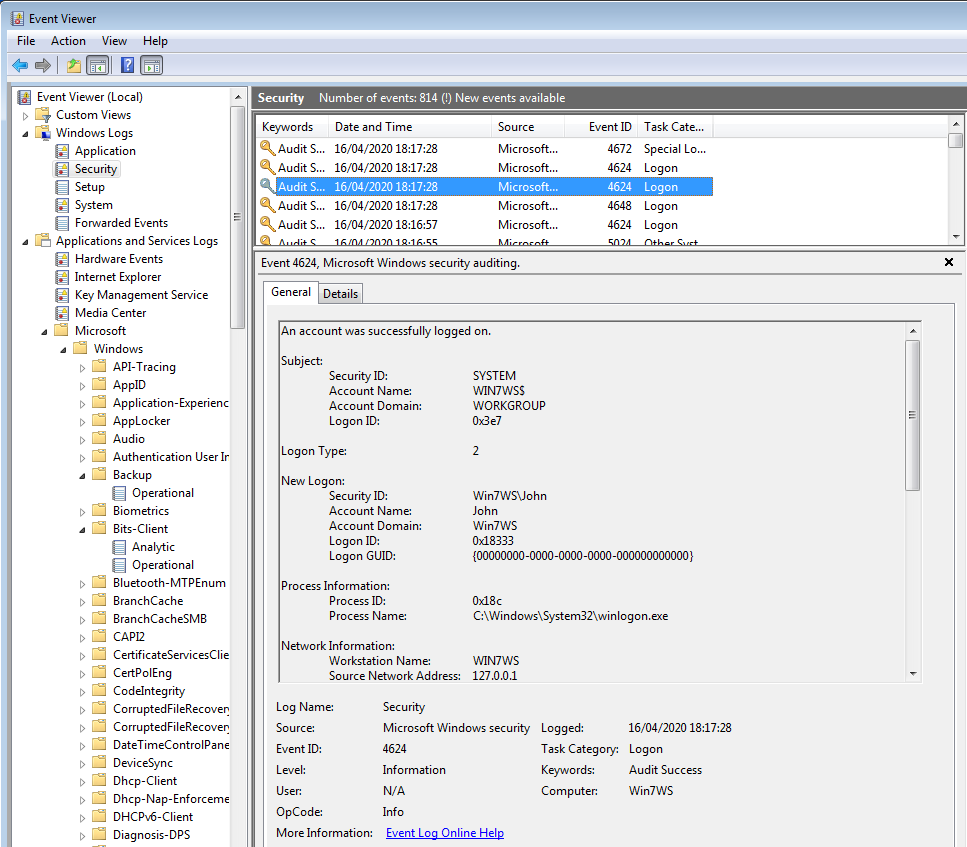
\includegraphics[scale=0.35]{images/evtx.png}
\end{frame}


\begin{frame}[fragile]
  \frametitle{2.3 Get support}
    \begin{itemize}
        \item Review logging policies
  \begin{lstlisting}[basicstyle=\tiny]
$ rip.pl -r SECURITY -p auditpol
.....
ystem:Other System Events                         S/F  
Logon/Logoff:Logon                                 S    
Logon/Logoff:Logoff                                S    
Logon/Logoff:Account Lockout                       S    
Logon/Logoff:IPsec Main Mode                       N    
Logon/Logoff:IPsec Quick Mode                      S    
Logon/Logoff:IPsec Extended Mode                   N    
Logon/Logoff:Special Logon                         N    
Logon/Logoff:Other Logon/Logoff Events             N    
Logon/Logoff:Network Policy Server                 S/F  
Object Access:File System                          N    
.....
  \end{lstlisting}
        \item Online:
            \begin{itemize}
                \item Microsoft TechNet
		\item \url{https://www.ultimatewindowssecurity.com/securitylog/encyclopedia/}
		\item \url{http://eventid.net/}
            \end{itemize}
    \end{itemize}
\end{frame}


\begin{frame}[fragile]
  \frametitle{2.4 Extracting and exploring event logs: Exercise}
  \begin{lstlisting}[basicstyle=\tiny]
Extracting event logs
---------------------
























_
  \end{lstlisting}
\end{frame}


\begin{frame}[fragile]
  \frametitle{2.4 Extracting and exploring event logs: Exercise}
  \begin{lstlisting}[basicstyle=\tiny]
Extracting event logs
---------------------

     mkdir evtx
     mkdir evtx/out

     mmls nps-2008-jean.raw
     sudo mount -o ro,offset=$((512*63)) nps-2008-jean.raw /media/sansforensics/casenps/

     cp /media/sansforensics/casenps/WINDOWS/system32/config/AppEvent.Evt evtx/
     cp /media/sansforensics/casenps/WINDOWS/system32/config/SecEvent.Evt evtx/
     cp /media/sansforensics/casenps/WINDOWS/system32/config/SysEvent.Evt evtx/
     ls -lh evtx/


Exploring event logs
--------------------









_
  \end{lstlisting}
\end{frame}


\begin{frame}[fragile]
  \frametitle{2.4 Extracting and exploring event logs: Exercise}
  \begin{lstlisting}[basicstyle=\tiny]
Extracting event logs
---------------------

     mkdir evtx
     mkdir evtx/out

     mmls image.raw
     sudo mount=o ro,offset=$((512*63)) image.raw/media/case1/

     cp /media/case1/WINDOWS/system32/config/AppEvent.Evt evtx/
     cp /media/case1/WINDOWS/system32/config/SecEvent.Evt evtx/
     cp /media/case1/WINDOWS/system32/config/SysEvent.Evt evtx/
     ls -lh evtx/


Exploring event logs
--------------------

     sudo apt install libevt-utils

     evtinfo evtx/AppEvent.Evt
     evtinfo evtx/SecEvent.Evt
     evtinfo evtx/SysEvent.Evt

     evtexport AppEvent.Evt | less
     evtexport SysEvent.Evt | less
  \end{lstlisting}
\end{frame}


\begin{frame}[fragile]
  \frametitle{2.4 Extracting and exploring event logs}
	\url{https://eventlogxp.com/}
    \includegraphics[scale=0.27]{images/evtx2.png}
\end{frame}


\begin{frame}[fragile]
	\frametitle{2.5 Example \texttt{.evtx}}
    \begin{itemize}
        \item Logon Success
  \begin{lstlisting}[basicstyle=\tiny]
$ evtxexport Security.evtx | less
.....
Event number          : 668
Written time          : Apr 15, 2019 12:58:33.650031000 UTC
Event level           : Information (0)
Computer name         : Win7WS
Source name           : Microsoft-Windows-Security-Auditing
Event identifier      : 0x00001210 (4624)
Number of strings     : 20
String: 1             : S-1-5-18
String: 2             : WIN7WS$
String: 3             : WORKGROUP
String: 4             : 0x00000000000003e7
String: 5             : S-1-5-21-3408732720-2018246097-660081352-1000
String: 6             : John
String: 7             : Win7WS
String: 9             : 2
.....
String: 17            : 0x0000018c
String: 18            : C:\Windows\System32\winlogon.exe
String: 19            : 127.0.0.1
  \end{lstlisting}
        \item Logon Fail
  \begin{lstlisting}[basicstyle=\tiny]
$ evtxexport Security.evtx | grep 4625
  \end{lstlisting}
    \end{itemize}
\end{frame}


\begin{frame}[fragile]
	\frametitle{2.5 Example \texttt{.evtx}}
    \includegraphics[scale=0.4]{images/f14_logonType.png}
\end{frame}


\begin{frame}[fragile]
  \frametitle{2.6 Other log files}
    \begin{itemize}
	\item \texttt{/Windows/setuplog.txt}
        \begin{itemize}
            \item Untill WinXP, when Windows is installed
        \end{itemize}
	\item \texttt{/Windows//Debug/netsetup.log}
        \begin{itemize}
            \item Untill WinXP, when Windows is installed
        \end{itemize}
	\item \texttt{/Windows/setupact.log}
        \begin{itemize}
            \item Graphical part of setup process
  \begin{lstlisting}[basicstyle=\tiny]
2019-04-05 11:39:56, Info  CBS Starting the TrustedInstaller main loop.
2019-04-05 11:39:56, Info  CBS TrustedInstaller service starts successfully.
2019-04-05 11:39:56, Info  CBS Setup in progress, aborting startup processing checks.
2019-04-05 11:39:56, Info  CBS Startup processing thread terminated normally
    \end{lstlisting}
	\end{itemize}
	\item \texttt{/Windows/setupapi.log}
  \begin{lstlisting}[basicstyle=\tiny]
/Windows/inf/setupapi.dev.log
/Windows/inf/setupapi.app.log
/Windows/inf/setupapi.offline.log
    \end{lstlisting}
	\item \texttt{/Windows/Tasks/SCHEDLGU.TXT}
        \begin{itemize}
            \item Task Scheduler Log
	\end{itemize}
    \end{itemize}
\end{frame}


\begin{frame}[fragile]
	\frametitle{2.7 Exercise: Automated tools}
  \begin{lstlisting}[basicstyle=\tiny]

     Example: Chainsaw
     =================
     
     wget https://github.com/WithSecureLabs/chainsaw/releases/
                  download/v2.10.1/chainsaw_all_platforms+rules.zip

     7z x chainsaw_all_platforms+rules.zip
     cd chainsaw
     chmod +x ./chainsaw_x86_64-unknown-linux-gnu
     git clone https://github.com/sbousseaden/EVTX-ATTACK-SAMPLES.git 

     ./chainsaw_x86_64-unknown-linux-gnu hunt EVTX-ATTACK-SAMPLES/ -s sigma/
          --mapping mappings/sigma-event-logs-all.yml | less


     [+] Loading detection rules from: sigma/
     [!] Loaded 3336 detection rules (490 not loaded)
     [+] Loading forensic artefacts from: EVTX-ATTACK-SAMPLES/Command 
         and Control, 2 (extensions: .evt, .evtx)



     Challenge: Hayabusa
     ===================

     https://github.com/Yamato-Security/hayabusa
  \end{lstlisting}
\end{frame}




